\documentclass[12pt]{article}
\usepackage[letterpaper, portrait, margin=1in]{geometry}
\usepackage{amsfonts}
\usepackage{amsmath}
\usepackage{listings}
\usepackage{graphicx}
\usepackage{breqn}
\pagenumbering{arabic}
\usepackage{subcaption}
\usepackage{amsthm}
\usepackage{cite}
\usepackage{makeidx}
\usepackage{hyperref}
\usepackage{comment}
\usepackage{algorithmicx}
%\graphicspath{{C:/Users/x92423/Documents/}}

\newcommand{\subsubsubsection}[1]{\paragraph{#1}\mbox{}\\}
\setcounter{secnumdepth}{4}
\setcounter{tocdepth}{4}
\begin{document}
\begin{titlepage}
	\begin{center}
		\vspace*{1cm}
		
		\textbf{\large Statistical Learning in Financial Markets}
		
		\vspace{0.5cm}
		Thesis Draft
		
		\vspace{1.5cm}
		
		\textbf{CDT Joseph Schlessinger \\ COL Grover LaPorte, LTC Tim Sikora, \& CPT Steven Morse}
		
		\vfill
		
		%A thesis presented for the degree of\\
		%Doctor of Philosophy
		
		\vspace{0.8cm}
		
		%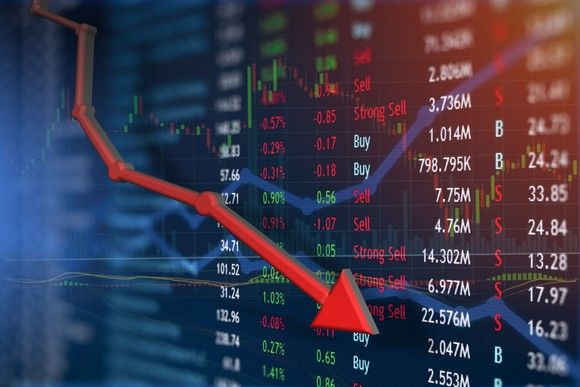
\includegraphics[width=0.8\textwidth]{stock.jpg}
		
		\vfill 
		Department of Mathematical Sciences\\
		United States Military Academy\\
		West Point, New York\\
		\today 
		
	\end{center}
\end{titlepage}

\tableofcontents
\newpage 

\begin{abstract}
	The day-to-day changes in the stock market are very difficult to predict; as such, many amateur investors rely on simple techniques that make no effort to time the market, such as dollar cost averaging. The goal of this project was to outperform dollar cost averaging by using an investment strategy informed by stock changes predicted by statistical learning. Our model focused on predicting the performance of a single stock. Our model was generally unsuccessful in predicting day-to-day changes, but was successful under certain cases. It appears that the complexities of the stock market cannot be modeled by basic linear models, but more complicated neural networks did show some progress. While modeling a regression proved to be very challenging, it was possible to get reasonable accuracy by modeling it as a classification problem. Moreover, the informed investment strategy was able to outperform dollar cost averaging in stagnant and bearish markets. As long as the stock market remains very difficult to predict, dollar cost averaging remains a simple yet effective investment strategy.
\end{abstract}

\section{Introduction}
There is an old saying that history has a way of repeating itself. Many believe this holds in the stock market. This project seeks to leverage this idea: based on the past performance of the stock market, can we predict what will happen next. We hope to create an informed investment strategy to beat dollar cost averaging, a common investment strategy explained later, by applying traditional time series analysis as well as newer methods of machine learning.

In the following report, we present a literature review encompassing the basics of investing, traditional time series analysis and machine learning. All of these broad topics play a central role in this project. 

We follow with an overview of the methods used in this project and the results. Finally, we present a plan for future work.

\section{Literature Review}
\subsection{Investment Basics}
Investing is a complicated subject. There are a number of different types of financial assets, trades, investment strategies, and risk measurements. For the purposes of this project, we will simplify financial markets significantly by focusing on a single type of security, stocks. 

\subsubsection{Stocks}
Stocks are the most basic element of the financial market. By owning a stock, in some sense you own part of a company. A public company is divided into shares through an initial public offering. If you own one share of Google, you own some small but measurable percent of that company.

A stock is a piece of some public company. A public company means it is traded publicly; anyone may purchase a share giving them partial ownership of the company. The stock market is open from 8:00 AM to 4:00 PM, at which point differing volumes of trading occur. 

\textbf{How is the market price set?} Most people have a vague idea of what determines the price of a stock at any given time: supply and demand. More precisely, the stock price is determined automatically by the exchange (e.g. NYSE) through a constant auction-like process consisting of ``asks'' and ``bids.'' An ask is a potential seller dictating a price that they are willing to sell at. A bid is a buyer dictating a price that they are willing to buy at. A computer then works to facilitate trades between all of the asks and the bids. The most recent price of a transaction is then the market price. This has profound effects on predictability, since a single stock price is a result of millions of decisions and a lot of human behavior; namely, traders speculation informed by a variety of factors drives decisions. \cite{stock}

\textbf{Different Markets Explored.} Below, I have summarized the markets explored throughout the project.

\begin{itemize}
	\item Bullish : in this market, the stock value increases. 
	
	\item Bearish : in this market, the stock value decreases.
	
	\item Noisy neutral : in this market, the stock value ends at the same point it starts. Between then, the stock both moves up and down. 
\end{itemize}

Although our study focuses on stocks, there are a number of other financial assets that make up the complicated financial markets. I have summarized a few of the most prominent ones below:

\begin{itemize}
	\item Bonds : A bond is like a share of debt. When an investor makes a loan to a borrower, the investor can divide up the loan among bonds, which others can then purchase and receive the interest from payback of the loan. 
	\item Commodities : Commodities are not strictly an investment term; they refer to anything that is an input in the production of something else. Some examples are oil, gold, and natural gas. Investors can trade on commodities by betting on whether the cost of such goods will go up or down.
	\item Options : A stock option gives an investor the option to buy or sell a stock at a certain price. A put option is a bet that the stock will fall or the right to sell at a certain price. A call option is a bet that the stock will rise or the right to to buy a stock at a certain price.
	\item Exchange-traded funds (ETFs) : An ETF tracks a stock index, commodity, bonds, or some combination of assets. Shares of ETFs are traded on an exchange like stocks.
	\item Mutual funds : A mutual fund is a pool of money collected for the purpose of investing in securities like stocks and bonds. The fund has a manage who allocates the funds money among different investments. 
\end{itemize}

\subsubsection{Dollar Cost Averaging}
Dollar cost averaging (DCA) is a popular investment strategy. It comes from the wisdom that the stock market is unpredictable; in other words, the investor has no way of knowing whether the stock value will increase or decrease. By investing some fixed amount at a regular interval, the investor averages out the risk and will gain, on average, whatever the stock makes. This phenomenon can be seen in Figure \ref{dca}. Dollar Cost Averaging is the standard of comparison for investment strategies. 

\textbf{Example.} Consider you want to invest in some stock X and you have a principal of \$12,000. If you were using DCA, you would pick some interval to invest at. If you decided on an interval of one month over a year, you would invest \$1,000 at the start of each month. However, on months where the stock is lower in price, you will buy more shares and when the stock is higher in price, you will buy fewer shares. The alternative is investing all of your money on the first day of the first month. DCA results in a lower average purchase price. Given the following equation for profit

$$\text{profit} = \text{number of shares } *( \text{current price} - \text{purchase price} )$$

it is obvious that a lower purchase price will increase profit. Figure \ref{dca} depicts this phenomenon. Obviously, the average purchase price with DCA is lower because the stock decreases after the first month. Note, DCA would be suboptimal if the stock only increased after the first month; in this case, it would be better to invest as a lump sum. Still, the unpredictability of the stock market and its tendency to fluctuate usually leads to DCA performing better than lump sum investing.

\begin{figure}[ht]
	\centering
	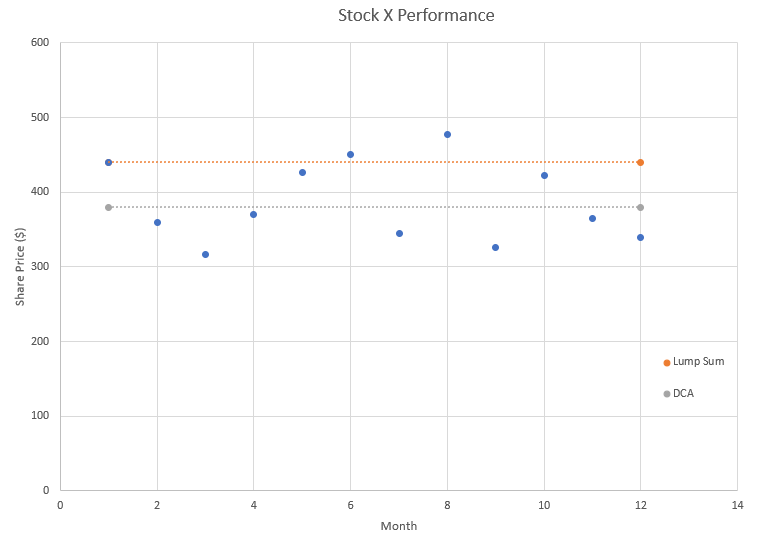
\includegraphics[width=.7\textwidth]{dca.png}
	\caption{Stock price at the beginning of each month is shown in blue. The orange line shows the average purchase price for a stock if it is invested as a lump sum at the beginning of the investment period. The gray line shows the average purchase price if the principal is divided up and invested at the beginning of each month according to dollar cost averaging with an interval of one month. \cite{dca}}
	\label{dca}
\end{figure}

With its simplicity, independence of market trends, and performance, dollar cost averaging is often used as the standard of comparison for investment strategies.

\subsection{Time Series Analysis}
Stock data examined over time forms a time series. Explicitly, we have some series $\{X_t\} = \{x_1, x_2, \dots, x_n\}$ where $x_t$ is a scalar corresponding to the price of a stock on day $t$. $x_t$ can also be a vector, where each day has multiple data points, such as the $t$th day's open price, close price, and volume traded. We are concerned with forecasting the price of a stock for the next day. Given $x_1 \dots x_k$, can we predict $x_{k+1}$?

We will now outline some basic properties of time series that we will reference throughout the paper.

\subsubsection{Stationary Models}  
A time series is stationary if it has similar statistical properties at $\{X_t\}$ and at $\{X_{t+h}\}$ for some $h$. For a more mathematically rigorous definition of stationary, we need to define some additional functions.

The mean function of $\{X_t\}$ is $\mu_X(t) = E(X_t)$. This refers to the average value of the time series or stock. The first requirement for stationarity is that $\mu_X(t)$ be independent of $t$. In the context of stocks, the time series around day 0 should have the same mean as the time series around day $n$. This rarely happens with financial data, which will be addressed later.

The second requirement has to do with the covariance of the time series. The covariance function of $\{X_t\}$ is defined as below, where $X_r$ and $X_s$ are subsets of the time series
$$\gamma _X(r,s) = \text{Cov}(X_r, X_s) = E[(X_r - \mu _X(r))(X_s - \mu_X(s))]$$

Our next requirement for a time series to be stationary is that $\gamma_X(t+h, t)$ is independent of $t$ for each $h$. 

\subsubsection{Trends, Seasonality, and Noise}
As a result, stock data as a time series is clearly not stationary, since it exhibits trends. Any time series which is, for example, steadily increasing, will not be stationary since its mean will also increase as you take subsets further into the series. A traditional way to decompose a time series is into a trend component, a seasonal component, and some random noise component. Thus, a time series can be decomposed in the following way
$$X_t = m_t + s_t + Y_t \ \ \ \ \ \ \text{additive decomposition}$$

where $m_t$ is the trend component, $s_t$ is the seasonal component, and $Y_t$ is some random stationary noise component. In Figure \ref{trends}, these components are on display. The plot titled purely random error is our random noise component; this is a stationary time series. The plots depict two types of trend, linear and nonlinear. A trend refers to some change to the data that occurs over time. As stocks generally increase overtime, there is clearly some trend involved in stock time series. Additionally, time series can have seasonality, seen in the bottom left of the figure. Anything that is cyclic can be represented as seasonality. As an example, if a stock increased at the beginning of the month, peaked in the middle, and then decreased before bottoming out at the end of the month, this would be a seasonality we would have to negate before applying time series analysis. The plot in the bottom right demonstrates an interaction of these additive terms, which is generally what financial data looks like. \cite[22]{timeseries}

\begin{figure}[ht]
	\centering
	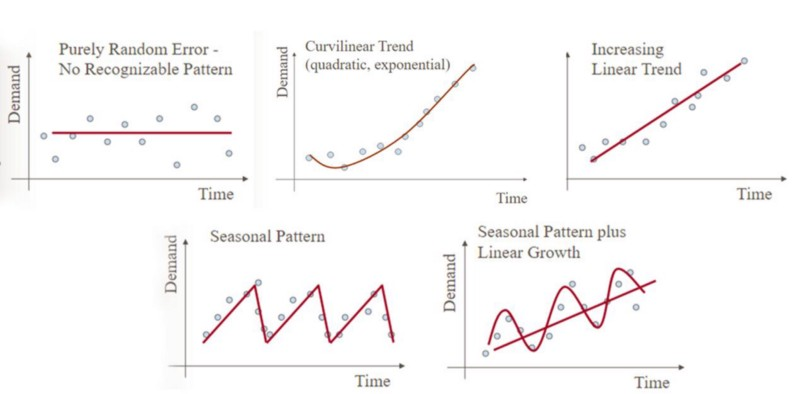
\includegraphics[width=.75\textwidth]{trend.jpeg}
	\caption{Trend and Seasonal components of a time series. \cite{trend}}
	\label{trends}
\end{figure}

\subsubsubsection{Trend and Seasonality Elimination by Differencing}

Many time series analysis models require a stationary time series. While we can account for this by attempting to estimate the trend and seasonality of the time series, in this case we will transform the data to eliminate trend and seasonality.

To eliminate trend, you can apply the difference operator $\nabla^d$ which lags the time series data by the past $d$ days.
$$\nabla^2 X_t = X_t - X_{t-1}=(1-B)X_t$$

where $B$ is the backward shift operator such that $BX_t = X_{t-1}$.

Thus, $$\nabla^t X_t = \nabla(\nabla(X_t)) = (1-B)(1-B)X_t = (1-2B+B^2)X_t = X_t-2X_{t-1}+X_{t-2}$$

This applies for some general $\nabla^d$. A similar technique can be used to negate seasonality by applying $\nabla_d$, where subscript $d$ instead refers to lagging by the value in the time series $d$ periods ago.

$$\nabla_d = X_t - X_{t-d} = (1-B^d) X_t$$

A more rigorous explanation can be found in \cite[22-32]{timeseries}. Given a stationary time series, we now briefly outline several classical methods for forecasting, i.e. predicting $x_{k+1}$ from $x_1 \dots x_k.$

\subsubsection{Moving Average}
Moving average models use the past forecast errors to model the time series and forecast. 

$$ x_{t} = c + \varepsilon_t + \theta_{1}\varepsilon_{t-1} + \theta_{2}\varepsilon_{t-2} + \dots + \theta_{q}\varepsilon_{t-q}$$

$\theta_q$ represents the weight for $\varepsilon_q$. An MA($q$) model considers the $q$ most recent data points. \cite[8.4]{forecasting}


\subsubsection{Autoregressive Models}
Autoregressive models use past values of the variable to predict future values of the variable. With financial data, the implication in using autoregressive models is the stock market repeats itself, and we can learn from the past what may happen in the future. \cite[8.3]{forecasting} The autoregressive model can be written as 

$$x_{t} = c + \phi_{1}x_{t-1} + \phi_{2}x_{t-2} + \dots + \phi_{p}x_{t-p} + \varepsilon_{t}$$

where $\varepsilon$ is white noise, $c$ is some intercept and $\phi_n$ is the weight associated with data point $y_n$. An AR($p$) model considers the most recent $p$ data points in the time series.

\subsubsection{ARIMA}
AutoRegressive Integrated Moving Average (ARIMA) combines moving average and auto-regression into one model. 

$$ x'_{t} = c + \phi_{1}x'_{t-1} + \cdots + \phi_{p}x'_{t-p} + \theta_{1}\varepsilon_{t-1} + \cdots + \theta_{q}\varepsilon_{t-q} + \varepsilon_{t} $$

$x'_t$ refers to the differenced series. This comes from the ``integrated'' part of the model; it is differenced. The general ARIMA model is of form ARIMA($p,d,q$) where $p$ is the order of the autoregressive part, $d$ is the degree of differencing, and $q$ is the order of the moving average part. \cite[8.5]{forecasting}

\section{Data}
We obtained all data for the project using the Yahoo! finance API. At the beginning of this research, we pulled all of the available data from each stock in the S\&P 500. The amount of data varies by stock. Older companies like GE have data going back to the late 1950s whereas newer companies like Google go back to the early 2000s. The code for this can be found in Appendix A.

\begin{figure*}[t!]
	\centering
	\begin{subfigure}[t]{0.3\textwidth}
		\centering
		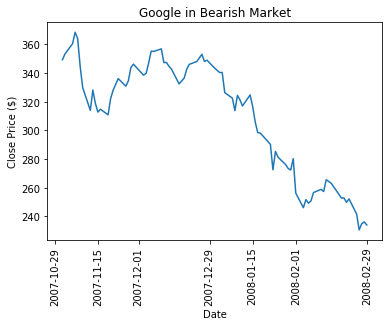
\includegraphics[width=\linewidth]{googBear.png}
		\caption{An example of Google stock in a bearish market.}
	\end{subfigure}%
	~ 
	\begin{subfigure}[t]{0.3\textwidth}
		\centering
		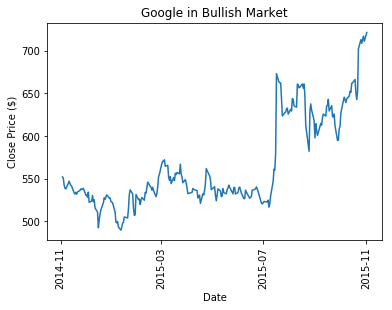
\includegraphics[width=\linewidth]{googBull.png}
		\caption{An example of Google stock in a bullish market.}
	\end{subfigure}
	~
	\begin{subfigure}[t]{0.3\textwidth}
		\centering
		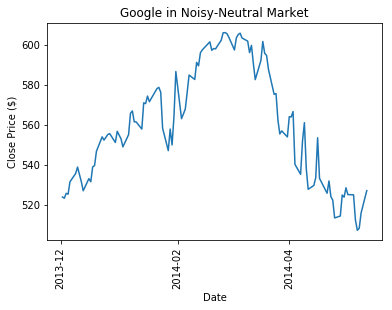
\includegraphics[width=\linewidth]{googNoisy.png}
		\caption{An example of Google stock in a noisy-neutral market.}
	\end{subfigure}
	
	\caption{This figure shows Google stock data over the different kinds of explored markets.}
\end{figure*}

\subsection{Features}
The available data for analysis is summarized below:

\begin{itemize}
	\item Close price - for a given day, this is the price that the stock ended at.
	\item Open price - for a given day, this is the price that the stock started at.
	\item Volume traded - for a given day, this is how many shares were traded
	\item High price - this is the daily high for the stock
	\item Low price - this is the daily low for the stock
\end{itemize}

\subsection{Time Lag}
The input vector was lagged at variable lengths. The number of days to lag was one of the many hyper-parameters in this process. Each feature was lagged for the same length.

\subsection{Differencing}
Stock data has a noticeable trend, and it is difficult to train a model on data with a trend. See Figure \ref{differencing} for a further explanation of the need for differencing.

We used a time differencing of one, which was sufficient and optimal for stationarity. A before and after of differencing can be found in Figure \ref{differencing2}. 

\begin{figure}
	\centering
	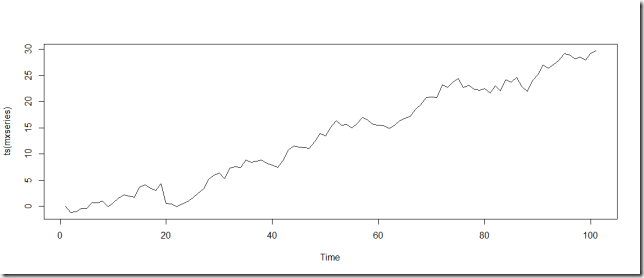
\includegraphics[width=.75\linewidth]{difference.png}
	\caption{Here is a time series with a clear upward trend. Imagine we trained a model on this data from 0 to 50 seconds and used 50 to 100 seconds as our test set. The inputs for our test set would be data values that the model had not trained on because the upward trend means the magnitude of the data increases over time. Differencing removes this issue by effectively recasting each data point in the context of the data preceding it.}
	\label{differencing}
\end{figure}

\begin{figure*}[t!]
	\centering
	\begin{subfigure}[t]{0.5\textwidth}
		\centering
		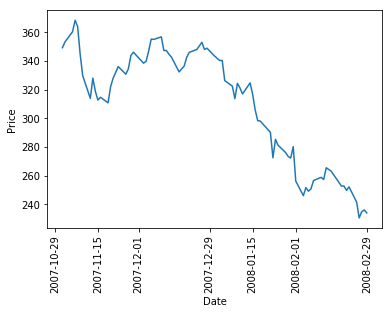
\includegraphics[width=\linewidth]{diff1.png}
		\caption{The time series data without any differencing.}
	\end{subfigure}%
	~ 
	\begin{subfigure}[t]{0.5\textwidth}
		\centering
		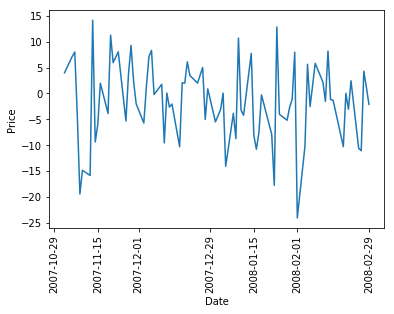
\includegraphics[width=\linewidth]{diff2.png}
		\caption{The time series data after a differencing with time delta 1.}
	\end{subfigure}
	\caption{This figure highlights the effect of differencing on stationarity.}
	\label{differencing2}
\end{figure*}

\subsection{Augmenting with Additional Stocks}
One of our intuitions was the correlation of stocks in the same sector or otherwise similar markets might be useful for our stocks. As such, our input vector also contained the lagged data for other stocks, to include closing price, opening price, volume traded, high and low.

With the multiple features for multiple stocks all lagged by the same number of days, the input grew very large. A typical simulation consisted of a few thousand days of training data with around 200 days of test data, and each day could easily have 100 data points, depending on the lag and additional stocks chosen. 

\section{Methods}
The research framework can be summarized in the following few steps:
\begin{enumerate}
	\item Using stock data, we build an input vector.
	\item We choose a machine learning model to train on all available data up until the beginning of the investment period.
	\item Using the trained model and the available data, predict the stock price of the next day.
	\item Given the model's prediction, decide to sell, buy or hold according to a strategy.
\end{enumerate}

\subsection{Machine Learning} 
Machine learning is a type of applied statistics that is often associated with mysterious terms like neural networks, artificial intelligence, and deep learning. However, it is important to note that these methods of machine learning are simply statistical models just as more rudimentary methods like linear regression are.

\subsubsection{Regression v. Classification}
Machine learning, in the context of prediction, breaks down into two main subsets: regression and classification. The distinction between the two subsets lies in the output type. Both share the same input of some set of data $\{(x_i, y_i)\}$. With regression $y_i \in \mathbb{R}$ whereas with classification, $y_i \in S$, where $S$ is the set of labels for the data.  \cite[9-10]{springer} When looking at stock time series data, a regression model would seek to forecast what the price of the stock will be the following day, while a classification model might seek to determine whether the stock will go up, down or stay the same. 

\subsubsection{Linear Models}
Linear models are one of the simplest approaches to prediction. Given a vector of inputs 
$\textbf{x} =  (x_1, x_2, \dots, x_n)^T$, a linear model predicts output by assuming the data is well predicted by a linear equation of the form 

$$\hat{Y} = \hat{\beta}_0 + \textbf{x}^T \boldsymbol{\hat{\beta}}$$

where $\hat{\beta_0}$ is the intercept for the data and $\boldsymbol{\hat{\beta}}$ is the vector of coefficients for the input vector $\textbf{x}$. \cite[11]{springer} 

We can estimate the coefficients (or ``weights'') using the method of least squares, which seeks to minimize the residual sum of squared error. 

With least squares, we select $\boldsymbol{\hat{\beta}}$ as the solution to the following optimization problem:

$$\boldsymbol{\hat{\beta}} = \text{arg} \min_\beta \sum_{i=1}^{N} \left(y_i - \beta_0 - \textbf{x}_i^T \boldsymbol{\hat{\beta}} \right)^2$$
\cite[42]{springer} This is a convex optimization problem and the solution can be written in closed form.


\textbf{Ridge Method}

One problem that can occur with least squares regression is poor prediction accuracy because of high variance. \cite[55]{springer} This is also known as over-fitting. A solution is to shrink the size of the regression coefficients by imposing a penalty on their size. This is called regularization. We make a simple modification of the least squares coefficient selection where we determine the coefficients according to the following formula: 
$$\boldsymbol{\hat{\beta}}_{\text{ridge}} = \text{argmin} \sum_{i=1}^{N} (y_i - \beta_0 -\textbf{x}_i^T \boldsymbol{\hat{\beta}})^2 + \gamma \sum_{j=1}^{p} \boldsymbol{\beta_j}^2$$
\cite[59]{springer}

Notice, the only difference between ridge and least squares is the penalty term for coefficient size, which is controlled by the tuning parameter $\gamma$. A large $\gamma$ will place a large penalty on parameter size. As $\gamma$ increases, the coefficients approach 0. Also, note that the following penalty represents the $L_2$ norm of $\boldsymbol{\beta}$ and it does not include $\beta_0$:

$$ \sum_{j=1}^{p} \boldsymbol{\beta_j}^2$$

\textbf{LASSO Method}


The Lasso (least absolute shrinkage and selection operator) method is another variant of least squares that employs a slightly different penalty. Coefficient selection goes according to the following equation:
$$\boldsymbol{\hat{\beta}}_{\text{Lasso}} = \text{argmin} \sum_{i=1}^{N} (y_i - \beta_0 - \textbf{x}_i^T \boldsymbol{\hat{\beta}})^2 + \gamma \sum_{j=1}^{p}|\boldsymbol{\beta_j}|$$

With Lasso, the penalty is $|\boldsymbol{\beta}|$ instead of $\boldsymbol{\beta}^2$ (the $L_1$ norm instead of the $L_2$ norm). One effect of using this different penalty is a sufficiently large $\gamma$ will lead to some coefficients equaling zero. The Lasso method thus does variable selection in addition to fitting a linear model. \cite[64]{springer}

Figure \ref{l2l1} explains the difference between the norms used as penalty in Ridge and Lasso. When optimizing the function, it is likely to intersect the $L_1$ norm on the axis, as seen on the right of Figure \ref{l2l1}, which leads to a coefficient value of zero. However, the function being optimized is more likely to intersect the $L_2$ norm somewhere not on the axis, giving a nonzero value for the coefficient

\begin{figure}
	\centering
	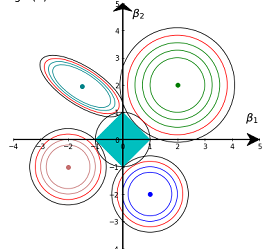
\includegraphics[width=.5\linewidth]{l1l2.png}
	\caption{Here we can see the $L_2$ and $L_1$ norm plotted on the same grid with different cost functions. The $L_2$ norm is the circle used in Ridge and the $L_1$ norm is the diamond used in Lasso. The various contour plots represent different cost functions. The optimal point for the constrained optimization problem is where the contours intersect the different norms. One can see that the contours tend to intersect the circle ($L_2$) not on the axes whereas they more often intersect the diamond ($L_1$) on the axes. This is why the $L_1$ norm leads to a greater likelihood of the coefficients being 0.}
	\label{l2l1}
\end{figure}

\subsubsection{Neural Networks}
Neural networks are a type of nonlinear statistical model. Neural networks have three parts: an input layer, which takes the same vector $\textbf{x}$, a hidden layer which performs an activation function, and an output layer. Assume we have $d$ input nodes, $m$ hidden layer nodes, and $n$ output nodes. The following explanation corresponds to Figure \ref{neuralnet}. Keep in mind, if this were a regression, there would be a single output node.

\begin{figure}[ht]
	\centering
	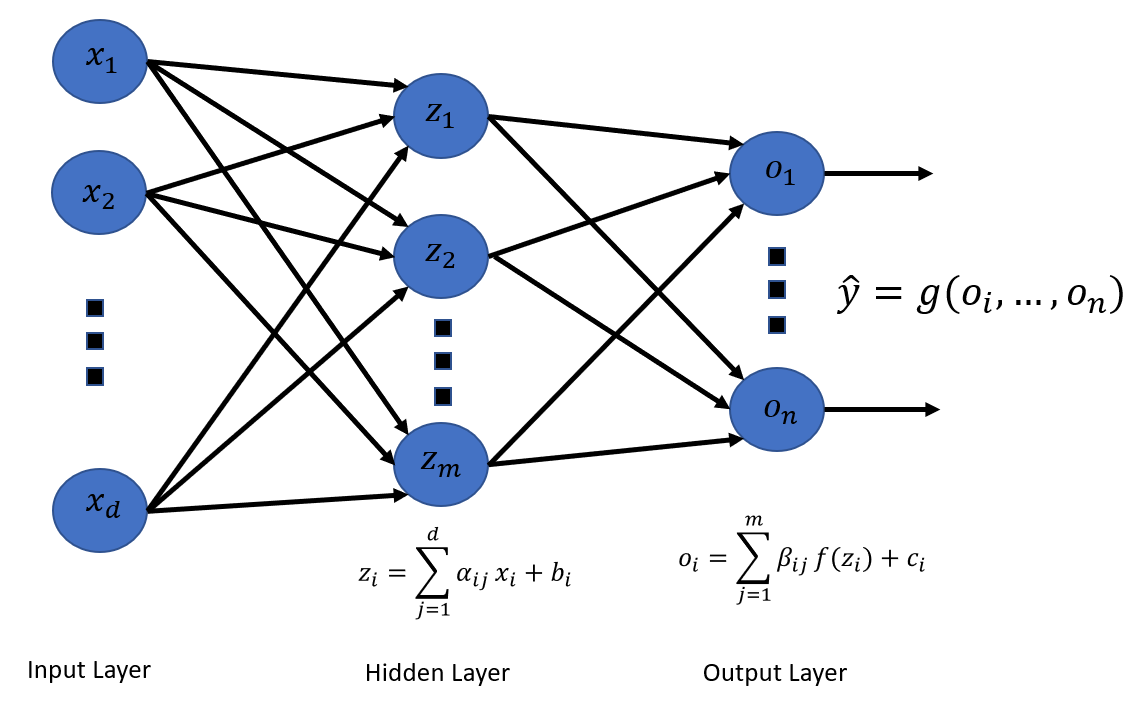
\includegraphics[width=.85\textwidth]{NeuralNetwork.png}
	\caption{This is a visual depiction of a general neural net. Note, for regression, there is a single output node. The description in the text generally follows this diagram. \cite{neural}}
	\label{neuralnet}
\end{figure}

This neural network takes an input $\textbf{x}$ with $d$ features. Each hidden layer node $z_i$ performs a linear transformation on the entire input layer given a vector of weights $\boldsymbol{\alpha_j}$ and some bias $\alpha_{0j}$. Bias in neural networks is simply an intercept for the vector of weights $\boldsymbol{\alpha_j}$. Each scalar weight $\alpha_{ji}$ corresponds to an input node $x_i$. \footnote{The hidden layer captures certain features of the model, but the weights and values do not have an obvious meaning. It is for this reason that neural networks are mysterious and often thought of as a black box.} The value of $z_j$ is simply the linear combination of the weights and input values:

$$z_j = \sum_{x=0}^{i}\boldsymbol{\alpha_{ji}} x_i + \alpha_{0j}$$

We then feed this set of hidden layer values $Z = \{z_j\}$ into the output layer.

Each output node has its own vector of weights $\boldsymbol{\beta_j}$ for each hidden layer nodes as well as a bias $\beta_{0j}$. The output node computes a linear combination of the hidden layer nodes and applies an activation function, $f$ to each hidden layer node value $z_i$.

$f$ is referred to as the activation function, which is often chosen to be the rectified linear unit (ReLU) picture in Figure \ref{relu}:

$$f(x) = \max(0,x)$$

Thus we have the following value for each output node: 

$$o_j = \sum_{i=0}^{J} \boldsymbol{\beta_{ij}} f(z_i) + \beta_{0j}$$

Finally the scalar from each output node is passed through a final output function $g$. For regression, the output function is typically the identity function applied to a single output node, so $g(a) = a$. \cite[350-351]{springer} For classification, on the other hand, each output node $o_i$ represents a label for the data. The output node with the largest value is the neural nets predicted label. The sigmoid function is often used to help transform the output node values into labels:

$$\sigma(v) = \frac{1}{1+e^{-v}}$$

The sigmoid function simply takes an input $v$ and maps it between 0 and 1, as seen in Figure \ref{sigmoid}. For a binary classification with a single output node, it follows that values above .5 would be classified as a 1 and values below .5 would be classified as a 0. Alternatively, you could do a binary classification with two output nodes and choose the output node with the larger value as the predicted classification.

\begin{figure*}[t!]
	\centering
	\begin{subfigure}[t]{0.5\textwidth}
		\centering
		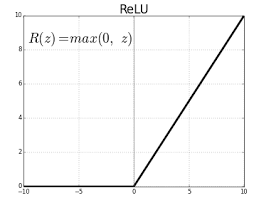
\includegraphics[width=\linewidth]{relu.png}
		\caption{The rectified linear unit is often used as the activation function in hidden layer nodes.}
		\label{relu}
	\end{subfigure}%
	~ 
	\begin{subfigure}[t]{0.5\textwidth}
		\centering
		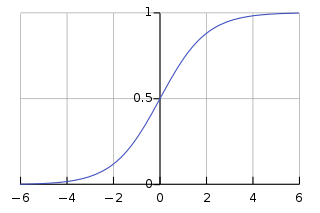
\includegraphics[width=\linewidth]{sigmoid.png}
		\caption{The sigmoid function is often used as a function in output layer nodes.}
		\label{sigmoid}
		
	\end{subfigure}

	\label{sigrelu}
\end{figure*}


In summary, we take some input vector $\textbf{x}$. Each hidden layer node takes the linear combination of learned weights and the value of each input node and outputs a scalar. Finally, the output layer node computes the linear combination of hidden layer weights and the hidden layer values along with some activation function. A final output function is applied and the neural network has made its prediction.

\subsubsection{Determining Coefficients}
While we have outlined the general model for a neural network, there are some undefined parameters. These are the weights that the neural network ``learns.'' We define the set of all weights as $\theta$, which consists of 

$$\{\boldsymbol{\alpha_i}, b_{0i}: i = 1, 2, \dots, m\}$$
$$\{\boldsymbol{\beta_j}, \beta_{0j}:  j= 1, 2, \dots, n\}$$

With regression, we can use sum-of-squared errors to measure fit and solve for coefficients. Note, this is the same measure of error used in the linear regression models. 
So, we determine the weights by solving the following squared error function, which sums over all $n$ data points. Let $F$ be the function representing the entire neural network.

$$\hat{\theta} = \text{arg} \min_\theta  \sum_{i=1}^{n} (y_{i} - F(x_i))^2$$ 

This is more complicated than with linear regression because we need to optimize a large multivariable summation. Moreover, the activation function may not be differentiable at all points, so it may not have a real gradient. In short, some neural network error functions can be optimized analytically, but this is very time-intensive. Thus, numerical methods are used to solve for the weights. Back propogation is one such short cut that is commonly used to optimize the error function. More details on back propogation can be found in \cite[354]{springer}. 

Using sum-of-squared errors leads to over-fitting in neural networks in the same way as least squares regression. Thus, neural networks can also include a penalty function in the same way that Ridge and Lasso do. 

It is important to understand that many elements of the neural network are customizable. You can have several hidden layers, you can add input nodes, hidden layer nodes, or output nodes. You can change the output function or the activation function. 

\subsection{Classification}
Reformulating the problem as a classification changes the error function. We can no longer use squared error because are outputs are categories. Instead, cross-entropy is used and the following error function is minimized: 

$$R(\theta) = \sum_{k=1}^{N} \sum_{i=1}^{N} (y_{ik} \log f_k(x_i))^2$$ 

The challenge for reformulating the stock problem as a classification problem is tuning the categories so that the classifier can be successful in general cases. We settled on three classes: buy, hold and sell. We ran tests to try and find the optimal division in percent yield; in other words, what percent yield range should be a buy, sell, and hold?

\subsubsection{Choosing Classes}
We experimentally determined the best intervals for the classes by training the model on a number of different intervals and seeing which performed best. Initially, we looked at the confusion matrices and the accuracy rate. We determined that the following mapping worked well, where $y$ is the percent yield: 

\[ \text{classify}(y) = \begin{cases} 
\text{sell} & y\leq -.2 \\
\text{hold} & -.2\leq y\leq .2 \\
\text{buy} & .2\leq y 
\end{cases}
\]

The confusion matrix is depicted in Figure \ref{confusion}.

\begin{figure}
	\centering
	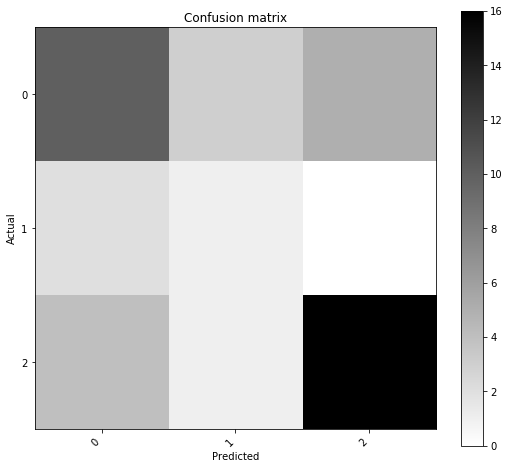
\includegraphics[width=.5\linewidth]{confusion.png}
	\caption{Here is the confusion matrix for our classification model. The cutoff between sell and hold was -0.2\% yield and the cutoff between hold and buy was a 0.2\% yieldsell.}
	\label{confusion}
\end{figure}



This is insufficient, however. Our overall goal is again the investment strategy. Overall accuracy may not be a tell-all because some mistakes are worse than others. Moreover, our investment strategy is not a direct reflection of the accuracy of the model. It is possible that a less accurate model holistically could give better results for the strategy. 
\subsubsection{Cross Validation}
Often the challenge with learning through statistical models is a shortage of data. We first have to partition this data set into a training and test set, as depicted in Figure \ref{test_train}. Additionally, there are a number of parameters that need to be chosen, but cannot be optimally solved for. These parameters are chosen through the cross validation process.

\begin{figure}[ht]
	\centering
	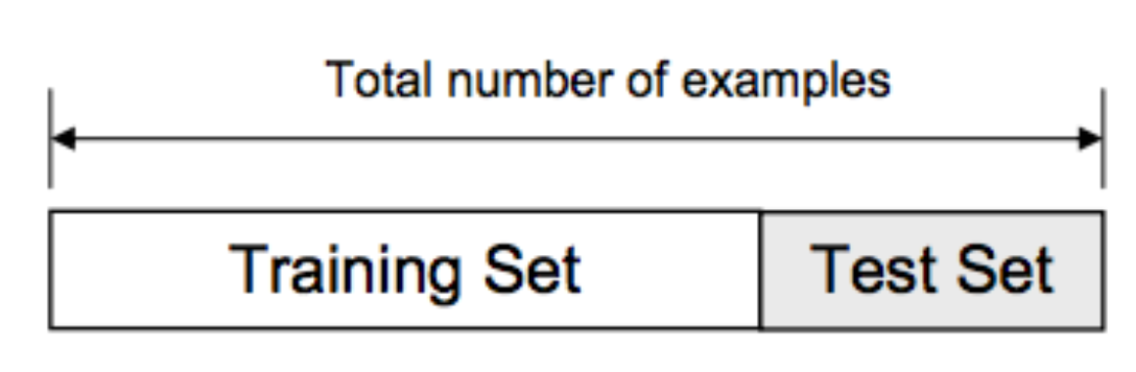
\includegraphics[width=.5\textwidth]{test_train.png}
	\caption{Training a model requires splitting data into a test set and a training set. \cite{kfold}}
	\label{test_train}
\end{figure}

This test set is untouched until the end when you evaluate the models performance on the data set. Thus, we already have a diminished data set when we are trying to train the model. There are useful methods to get the most out of your training set and tune hyper-parameters One such method is K-fold cross validation graphically depicted in Figure \ref{kfold}. K-fold could be used to select $\lambda$ in Ridge regression, before training the model on the entire training set using the determined optimal $\lambda$.

\begin{figure}[ht]
	\centering
	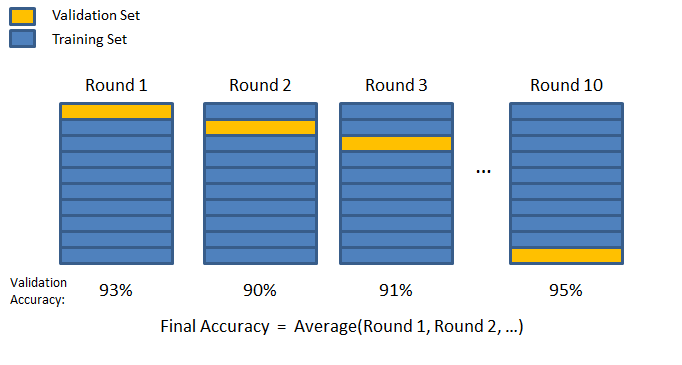
\includegraphics[width=.5\textwidth]{kfold.png}
	\caption{This figure depicts a K fold cross validation where $k=10$. \cite{kfold}}
	\label{kfold}
\end{figure}

$K$-fold cross validation takes the training data and partitions it into $K$ segments. It then trains the model on $K-1$ segments, and evaluates the fit of the model on the remaining segment. It runs $K$ rounds choosing a different validation segment each time. The average of the $K$ rounds is taken as the score. The entire process of splitting data and validating can be seen in Figure \ref{test_train_validate}.

\begin{figure}[ht]
	\centering
	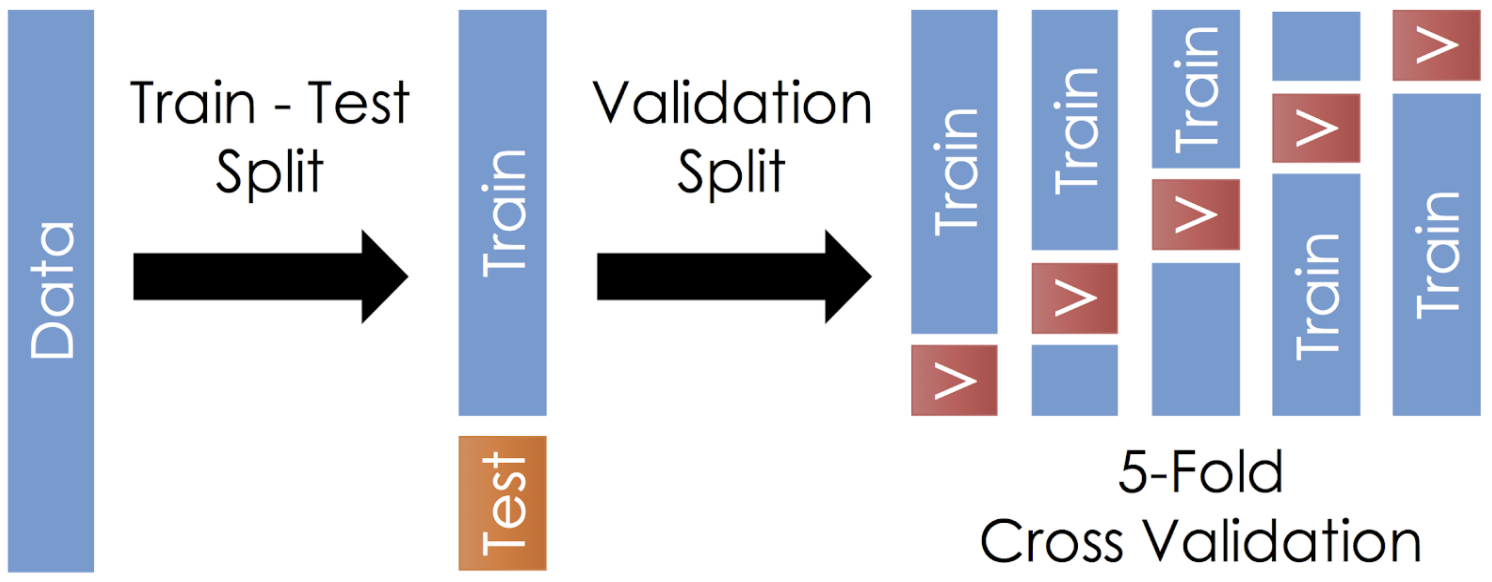
\includegraphics[width=.5\textwidth]{test_train_validate.png}
	\caption{This figure depicts the entire process of training a model. It demonstrates a $K$-fold cross validation where $k=10$. \cite{kfold2}}
	\label{test_train_validate}
\end{figure}

\subsection{The Strategy}
The prediction engine is the important mathematical part of the project, but the investment strategy is similarly important because the final goal was to compare to dollar cost averaging. 

\subsubsection{Practical Assumptions}
In an effort to transform the financial world into a more reasonable object for academic research, we have made a few simplifying assumptions.
\begin{itemize}
	\item Trades occur instantly and at the beginning of the day. The investment algorithm purchases at the exact price the stock closed at the previous day. This is unrealistic to some extent because in order to purchase some number of shares at some price, there has to be another owner willing to sell those shares at that price, which is not always the case. However, this assumption is consistent across both the statistical investment methods and dollar cost averaging standard of comparison.
	
	\item There is no transaction fee, which is not the case when trading. Typically, investors pay some fixed fee to the brokerage firm for completing the transaction. Again, because this is a consistent assumption in the dollar cost average baseline, this will not affect the comparison.
	
	
	\item We are assuming that the stock market has some degree of predictability. In particular, we assume that the future value of a stock can generally be predicted by the recent history of the stock.
\end{itemize}

\subsubsection{Dollar Cost Averaging}
The dollar cost averaging strategy is uninformed. Given an interval for investment, the dollar cost averaging strategy was programmed to divide the initial principal into the number of days of investment, and buy an equal amount each day of investment.

\subsubsection{Yield Estimation Proportionality Investing}
The basis of our investment strategy was to invest an amount of money that was proportional to the expected yield of the stock. If the stock is supposed to go up a lot, buy a lot. This is a notably short-sighted strategy, which has its pros and cons. In the case of the classification variation, the goal was to scale the investment amount with the classifer's confidence in its classification. 

\subsubsection{Short-Sighted Investment Strategies}
The short-sighted nature of the investment strategy was founded in a number of assumptions summarized below.
\begin{itemize}
	\item The goal of the project was to compete with dollar cost averaging, which basically follows the market. So, we knew it would be possible to beat dollar cost averaging in markets where the stock goes down or stays the same. Our strategy has the flexibility to sell stocks, while dollar cost averaging can only increase its stake. One consequence of the nature of dollar cost averaging is it is near optimal in a bullish market. In other words, when the stock is going up, dollar cost averaging is doing well because its position gets larger and larger. This leaves two options to outperform dollar cost averaging:
	\begin{enumerate}
		\item Invest heavier than dollar cost averaging earlier in the investment period 
		\item Capitalize on the local maximums and minimums in the stock. 
	\end{enumerate}

	 The first option was not possible because our method has some averaging as well; we reserve a maximum investment amount each day to avoid spending all the money early in the investment period. So, to beat dollar cost averaging, we would have to exploit the second option. These local maximums and minimums can be day to day; there is potential for earning every time the stock fluctuates. This was the motivation for the short-sighted strategy.
	 
	 \item Forecasting models typically get substantially worse as they are projected further out. Thus, we thought we would be most accurate at predicting the near future. 
	 
	 \item The model, and limitations in compute power, forced us to focus on microtrends in the market, rather than macrotrends. In predicting the future, we would look on the scale of the past week or two, rather than the past few months. It would be difficult to project further out and capture long term trends with such a recent input vector.
	 
	 \item Lastly, we wanted to have a reasonably fair comparison. We tried to model the strategy after dollar cost averaging. If we gave our model the same amount of money to play with, but the option to invest less or potentially sell, would it be better than dollar cost averaging? It was difficult to make the investment strategy sufficiently comparable to dollar cost averaging specifically because our strategy had the unfair advantage of being able to sell. Any complexity in the strategy both made the comparison to dollar cost averaging difficult as well as confused the effects of the machine learning that was informing the model.
\end{itemize}

The strategy is summarized below.

\begin{enumerate}
	\item Allocate some budget $d$ out of your total principal to invest each day.\footnote{This is somewhat arbitrary. We found that without allocating a budget, the strategy invested a lot of money up front and did not invest later on. As our baseline for comparison is dollar cost averaging which invests a fixed amount at a certain interval, we allocated a daily amount to invest for a more equal comparison.}
	\item Estimate $x_{n+1}$ using a model. Compute the estimated percent yield $\hat{p} = \frac{\hat{x_{n+1}}-x_n}{x_n}$. In the case of classification, convert the classification into a percentage of positive or negative confidence.
	\item If $\hat{p} > 0$, purchase the following dollar amount worth of stock: $\alpha \cdot \hat{p} \cdot d$. $\alpha$ is a hyper-parameter that is set experimentally based on the most successful simulations.
	
	If $\hat{p}> 0$, then sell the following number of shares: $\beta \cdot \hat{p} \cdot \text{shares owned}$
\end{enumerate}

\subsection{The Simulation}
Below, we have listed the variables for the simulation:
\begin{itemize}
	\item \textit{stock} - the stock in the S\&P 500 that will be modeled and invested in
	\item \textit{timeframe} - the period of time in the past that the investment will take place during
	\item \textit{principal} - the amount of money the simulation starts with
	\item \textit{trainingData} - the amount of training data to consider. If left blank, the model will attempt to fit to all of the available data. Otherwise, it will used the preceding $n$ days
	\item \textit{validationFreq } - tells the model how often to retrain the model, reselect parameters, and cross validate.
	\item \textit{parameterRange } - tells the model which parameter values to try when it is selecting through cross validation
	\item \textit{$\alpha$} - the tuning parameter for purchasing stocks
	\item \textit{$\beta$} - the tuning parameter for selling stocks
\end{itemize}

\section{Results}
The models were compared based on a number of investment periods: bullish, bearish, and noisy neutral. 

\begin{center}
	\begin{tabular}{|l | c | r |}
		\hline 
		Figure & Prediction Method & Market Type \\ \hline 
		Figure \ref{{fig:goog-dca-ridge-mlp-2010-12-02--2011-12-12-alphas--30-trainlength-500-performanceplot} & Regression & Noisy-Neutral \\ \hline
		Figure \ref{fig:goog-dca-ridge-mlp-2013-12-02--2014-05-12-alphas--30-trainlength-500-performanceplot} & Regression & Noisy-Neutral \\ \hline
		Figure \ref{fig:goog-dca-ridge-mlp-2007-11-01--2008-11-01-alphas--30-trainlength-500-performanceplot} & Regression & Bearish \\ \hline
		Figure \ref{fig:victory} & Classification & Bullish \\ \hline
		Figure \ref{fig:goog-dca-mlpclass-2014-11-02--2015-11-02--performanceplot} & Classification & Bullish \\ \hline
		Figure \ref{fig:goog-dca-mlpclass-2007-11-01--2008-03-01--performanceplot} & Classification & Bearish \\ \hline
		Figure \ref{class-steady} & Classification & Noisy-Neutral \\ \hline 
	\end{tabular}
\end{center}


\subsection{Regression}

\begin{figure}
	\centering
	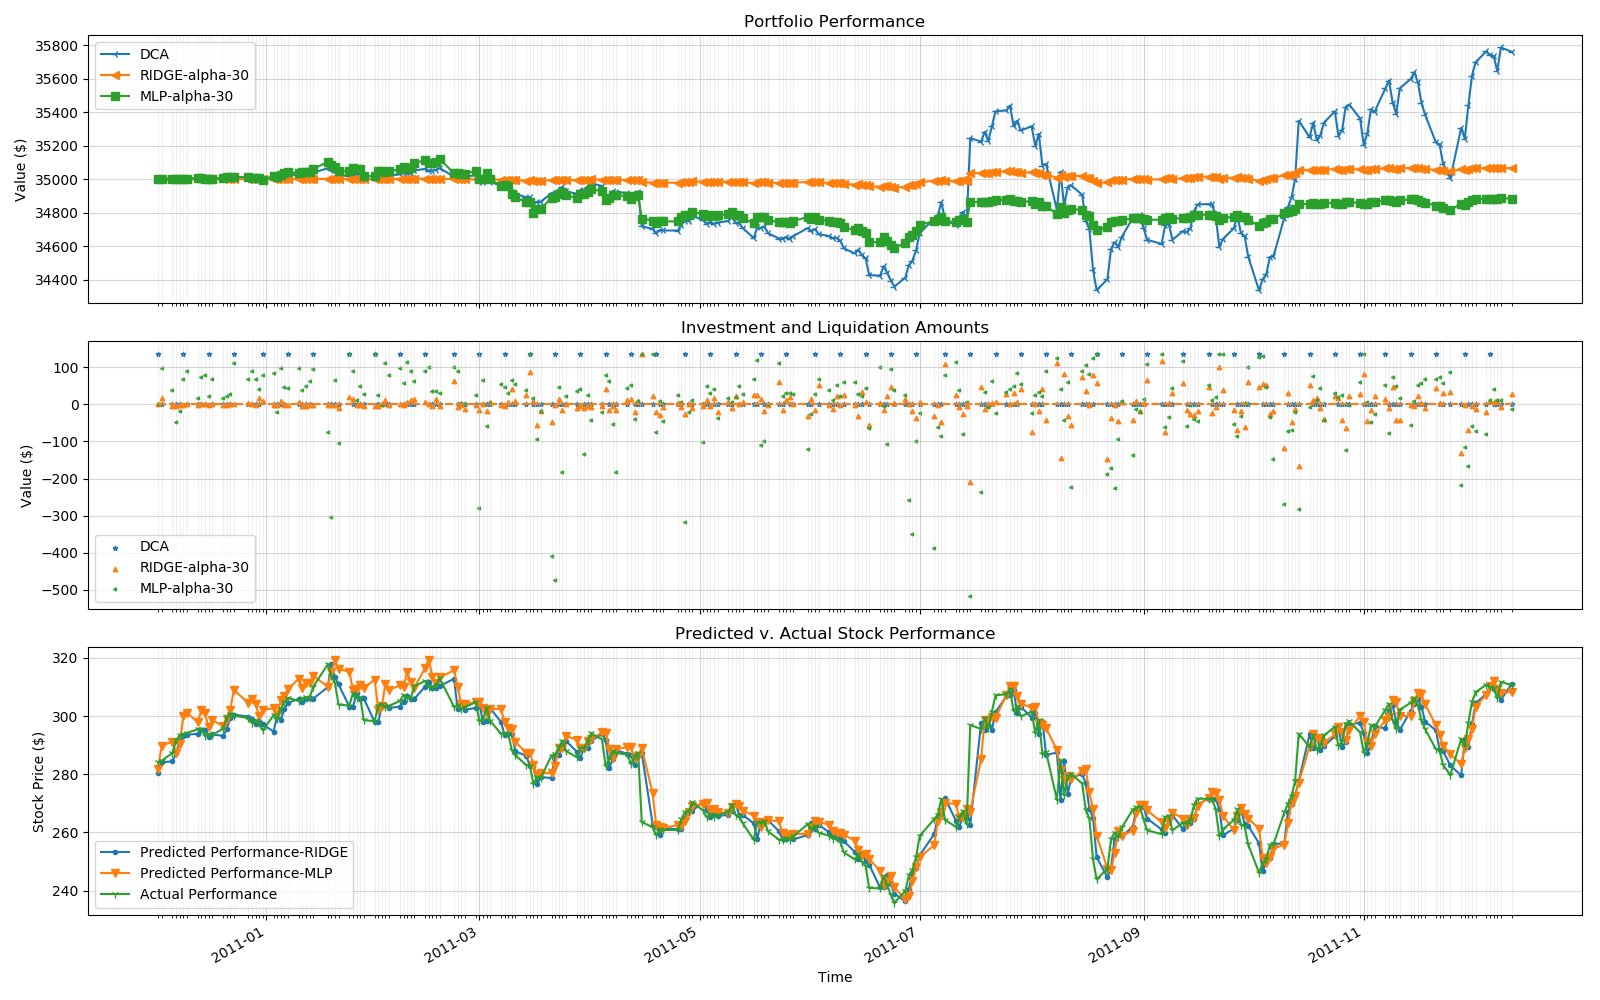
\includegraphics[width=\linewidth]{../Results/GOOG-DCA-RIDGE-MLP-2010-12-02--2011-12-12-alphas--[30]-train_length-500-performanceplot}
	\caption{Here is an example of a time period in which the stock goes up slightly. Ridge and the multi-layer perceptron lose to dollar cost averaging, which mirrors the amrket that increases. Here, the regression based models clearly are unable to take advantage of small gains with basically no change.}
	\label{fig:goog-dca-ridge-mlp-2010-12-02--2011-12-12-alphas--30-trainlength-500-performanceplot}
\end{figure}

\begin{figure}
	\centering
	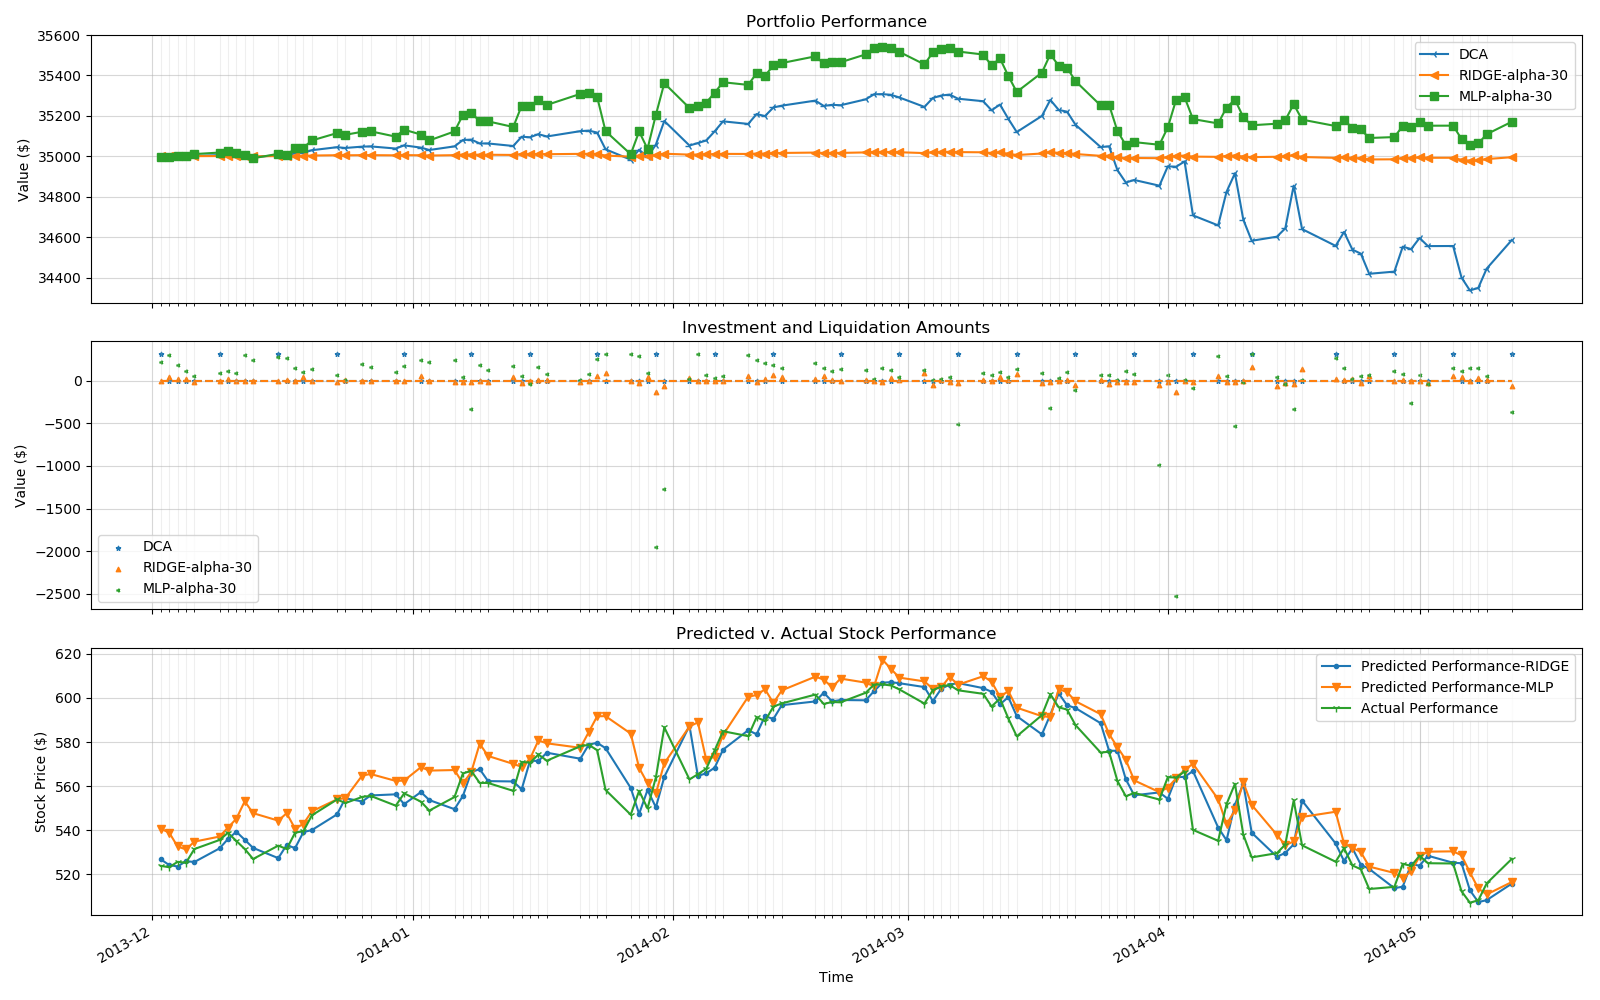
\includegraphics[width=\linewidth]{../Results/GOOG-DCA-RIDGE-MLP-2013-12-02--2014-05-12-alphas--[30]-train_length-500-performanceplot}
	\caption{Here is an example of a noisy steady market. Dollar cost averaging performs worst here. Multi layer perceptron is able to take advantage of early rises, and by selling its position when the stock is going down, it is able to weather some of the markets fall.}
	\label{fig:goog-dca-ridge-mlp-2013-12-02--2014-05-12-alphas--30-trainlength-500-performanceplot}
\end{figure}

\begin{figure}
	\centering
	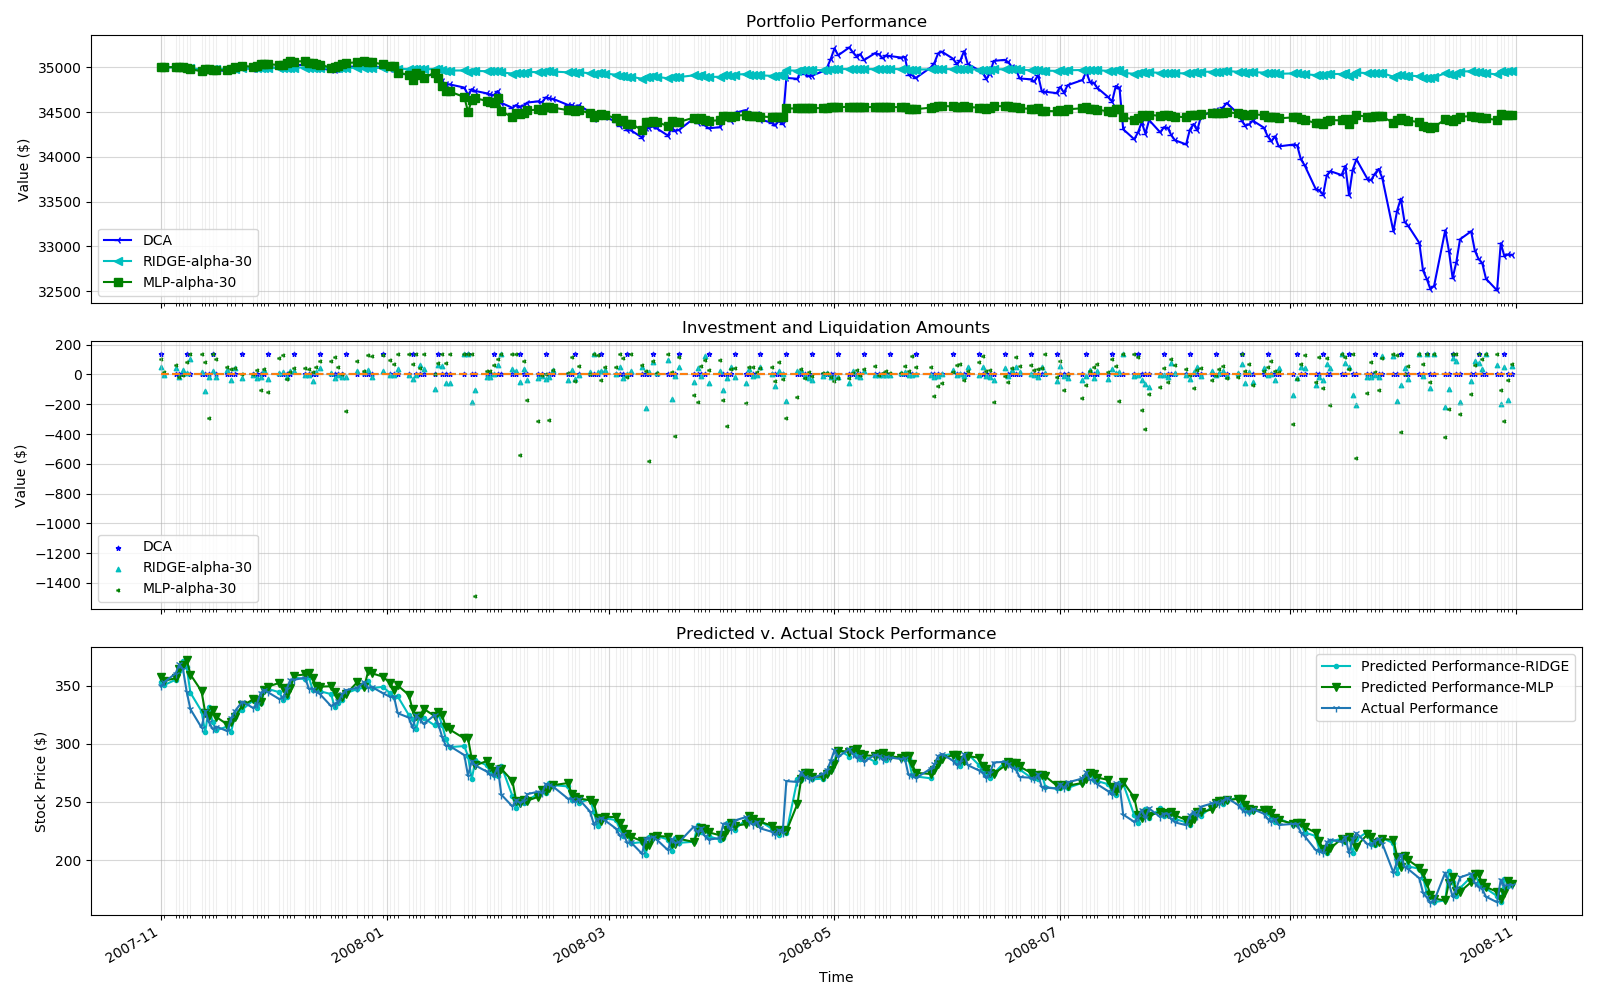
\includegraphics[width=\linewidth]{../Results/GOOG-DCA-RIDGE-MLP-2007-11-01--2008-11-01-alphas--[30]-train_length-500-performanceplot}
	\caption{Here is a declining market. Dollar cost averaging consistently performs worse here because it is unable to sell and has a heavy position in a declining stock.}
	\label{fig:goog-dca-ridge-mlp-2007-11-01--2008-11-01-alphas--30-trainlength-500-performanceplot}
\end{figure}





\subsection{Classification}

\begin{figure}
	\centering
	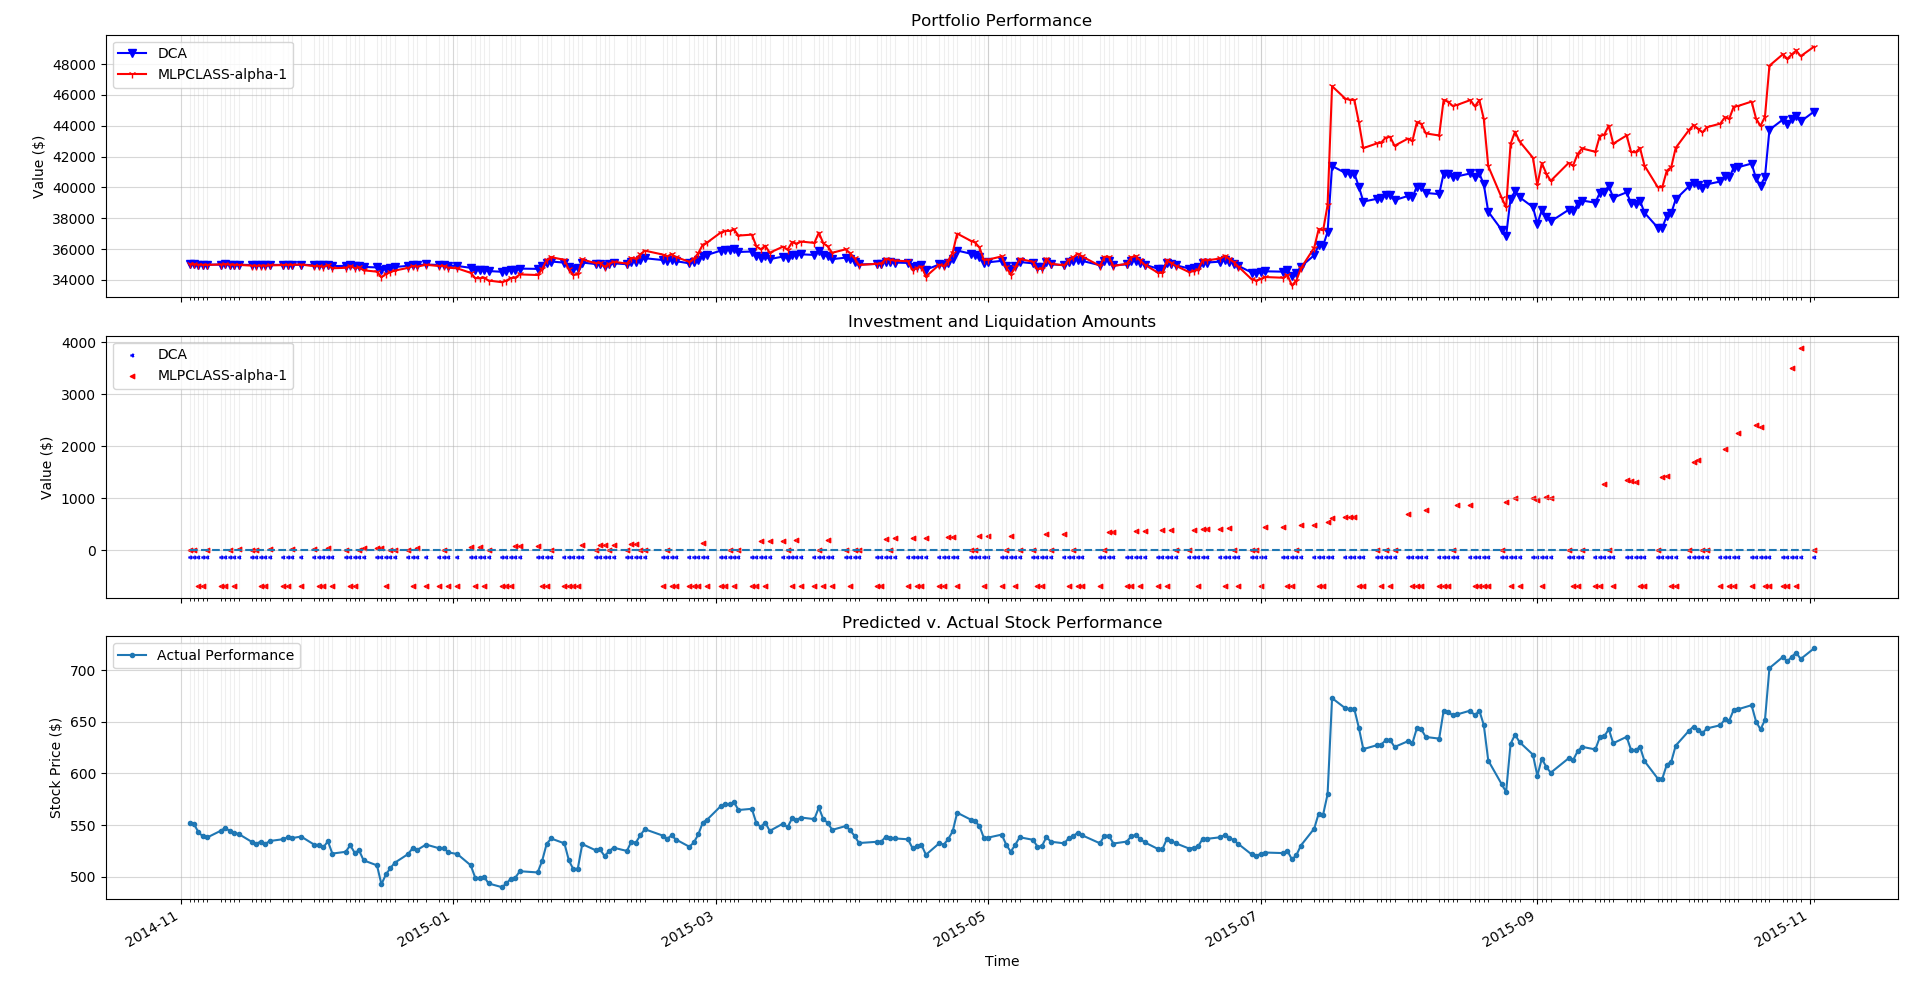
\includegraphics[width=\linewidth]{../Results/victory}
	\caption{This shows the mlp classifier outperforming dollar cost averaging in a bull market, which was the goal at the start. Unfortunately, this result was not largely reproducible.}
	\label{fig:victory}
\end{figure}

\begin{figure}
	\centering
	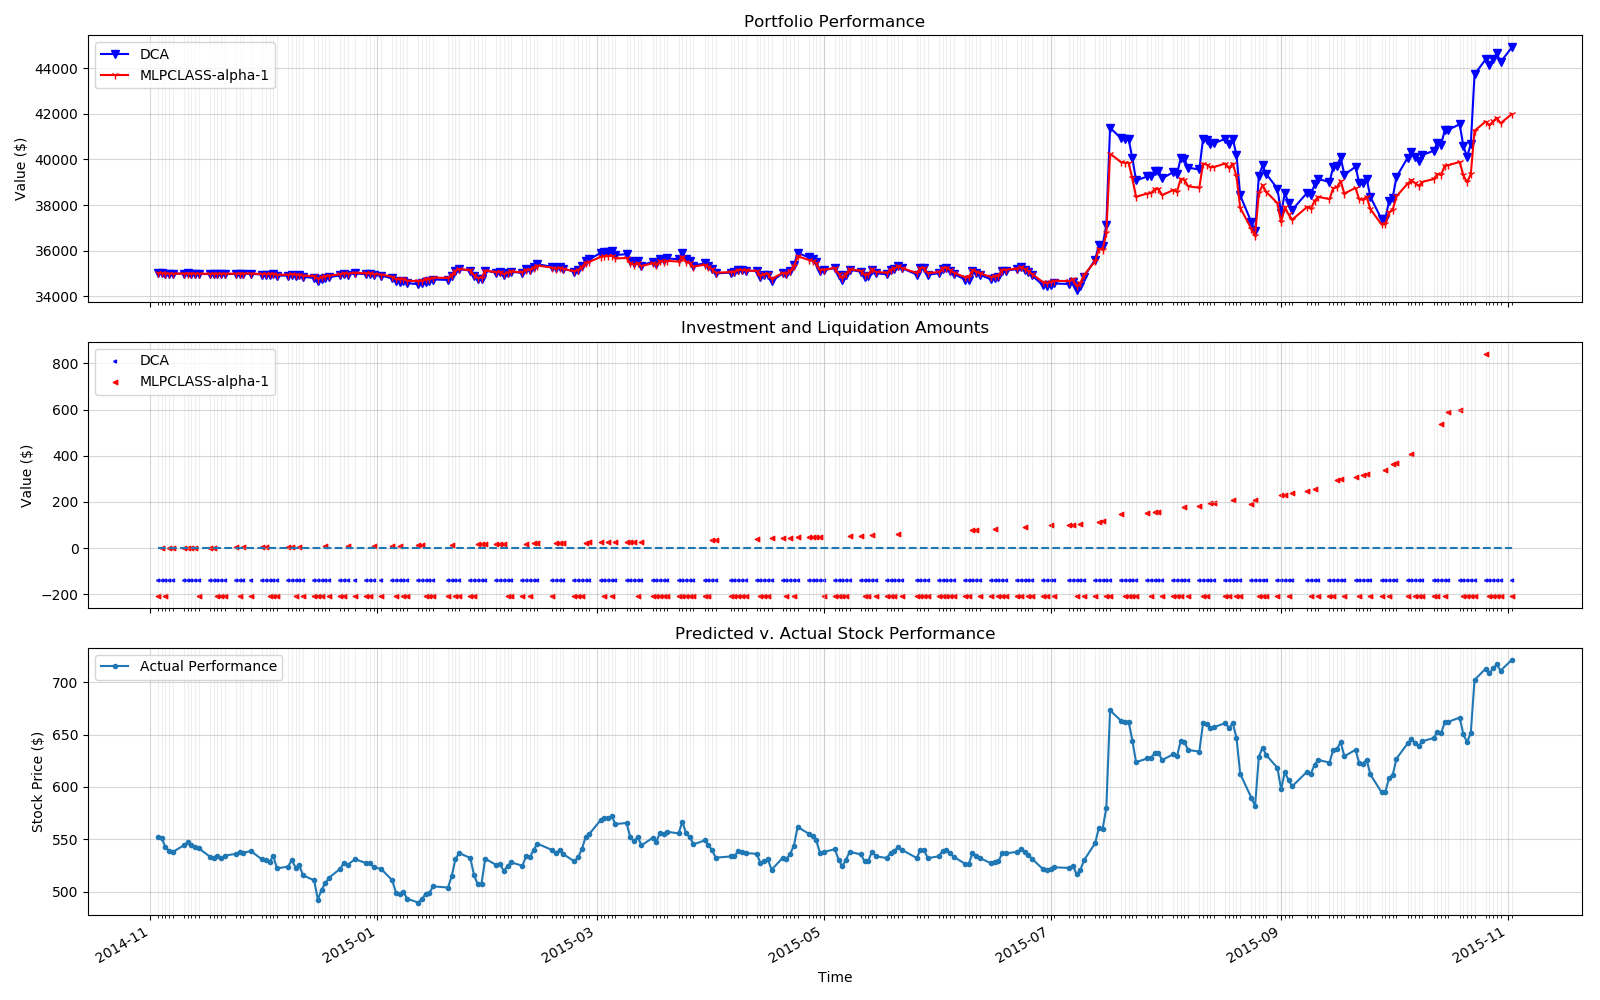
\includegraphics[width=\linewidth]{../Results/GOOG-DCA-MLPCLASS-2014-11-02--2015-11-02--performanceplot}
	\caption{This shows the multi layer perceptron classifier in a bullish market losing to dollar cost averaging. This uses a more conservative investment strategies, where you invest or sell \%30 of assets based on the classification.}
	\label{fig:goog-dca-mlpclass-2014-11-02--2015-11-02--performanceplot}
\end{figure}



\begin{figure}
	\centering
	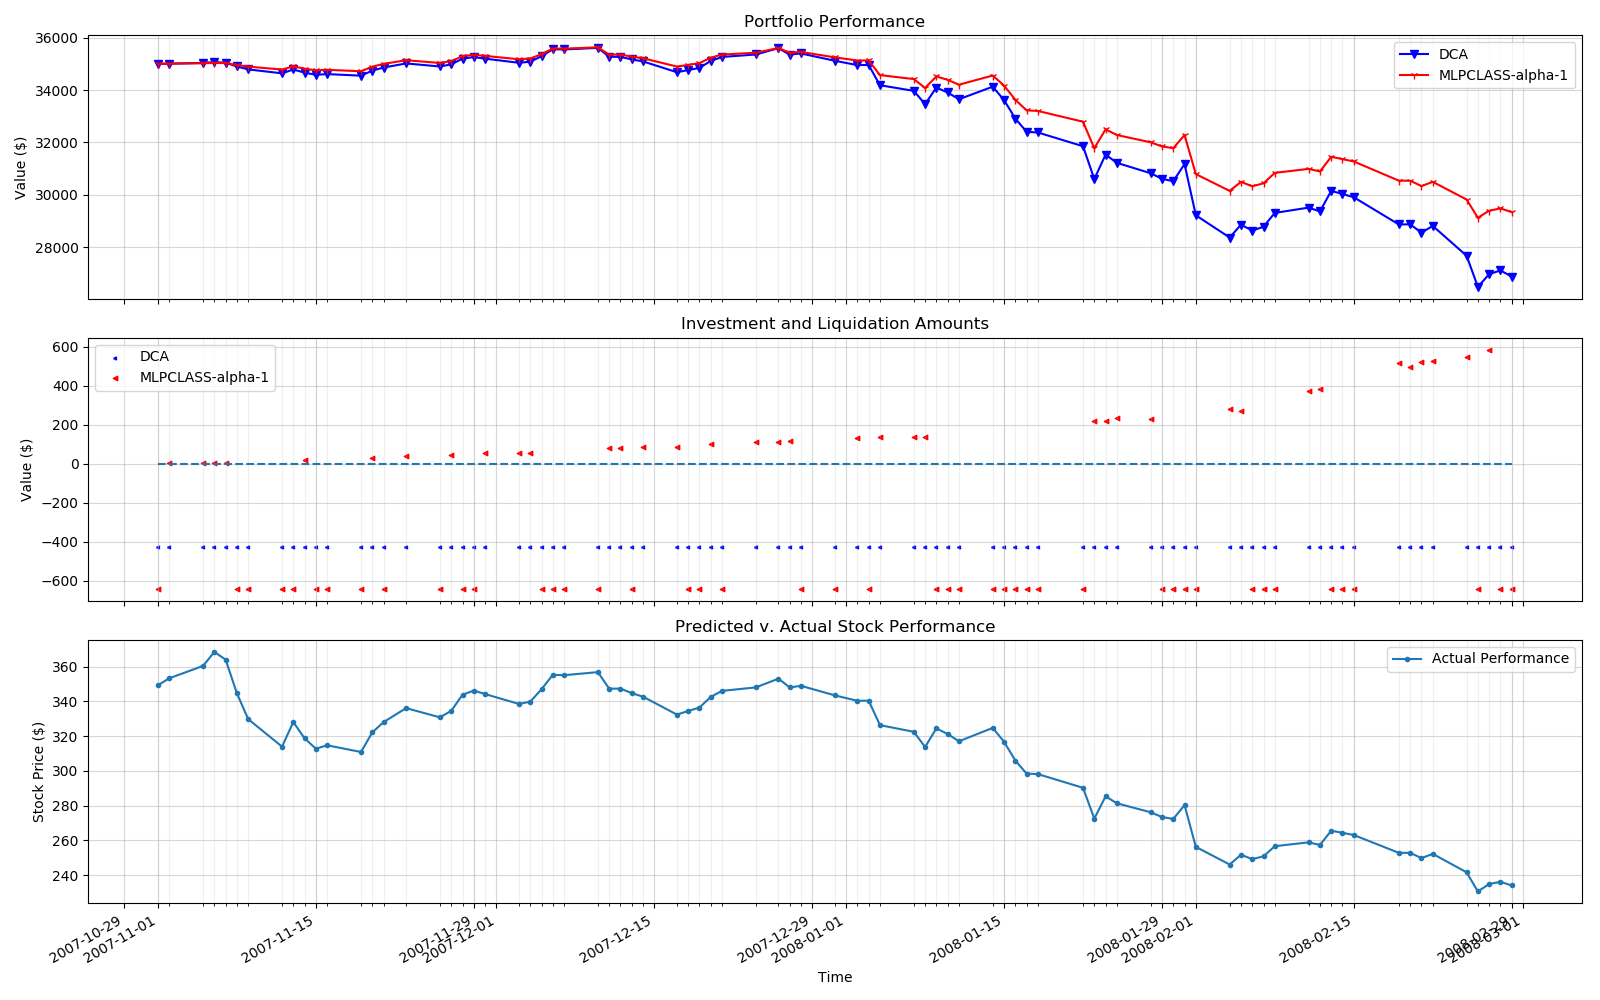
\includegraphics[width=\linewidth]{../Results/GOOG-DCA-MLPCLASS-2007-11-01--2008-03-01--performanceplot}
	\caption{This shows a bearish market. With the conservative investment strategy, MLP outperforms DCA.}
	\label{fig:goog-dca-mlpclass-2007-11-01--2008-03-01--performanceplot}
\end{figure}



\begin{figure}
	\centering
	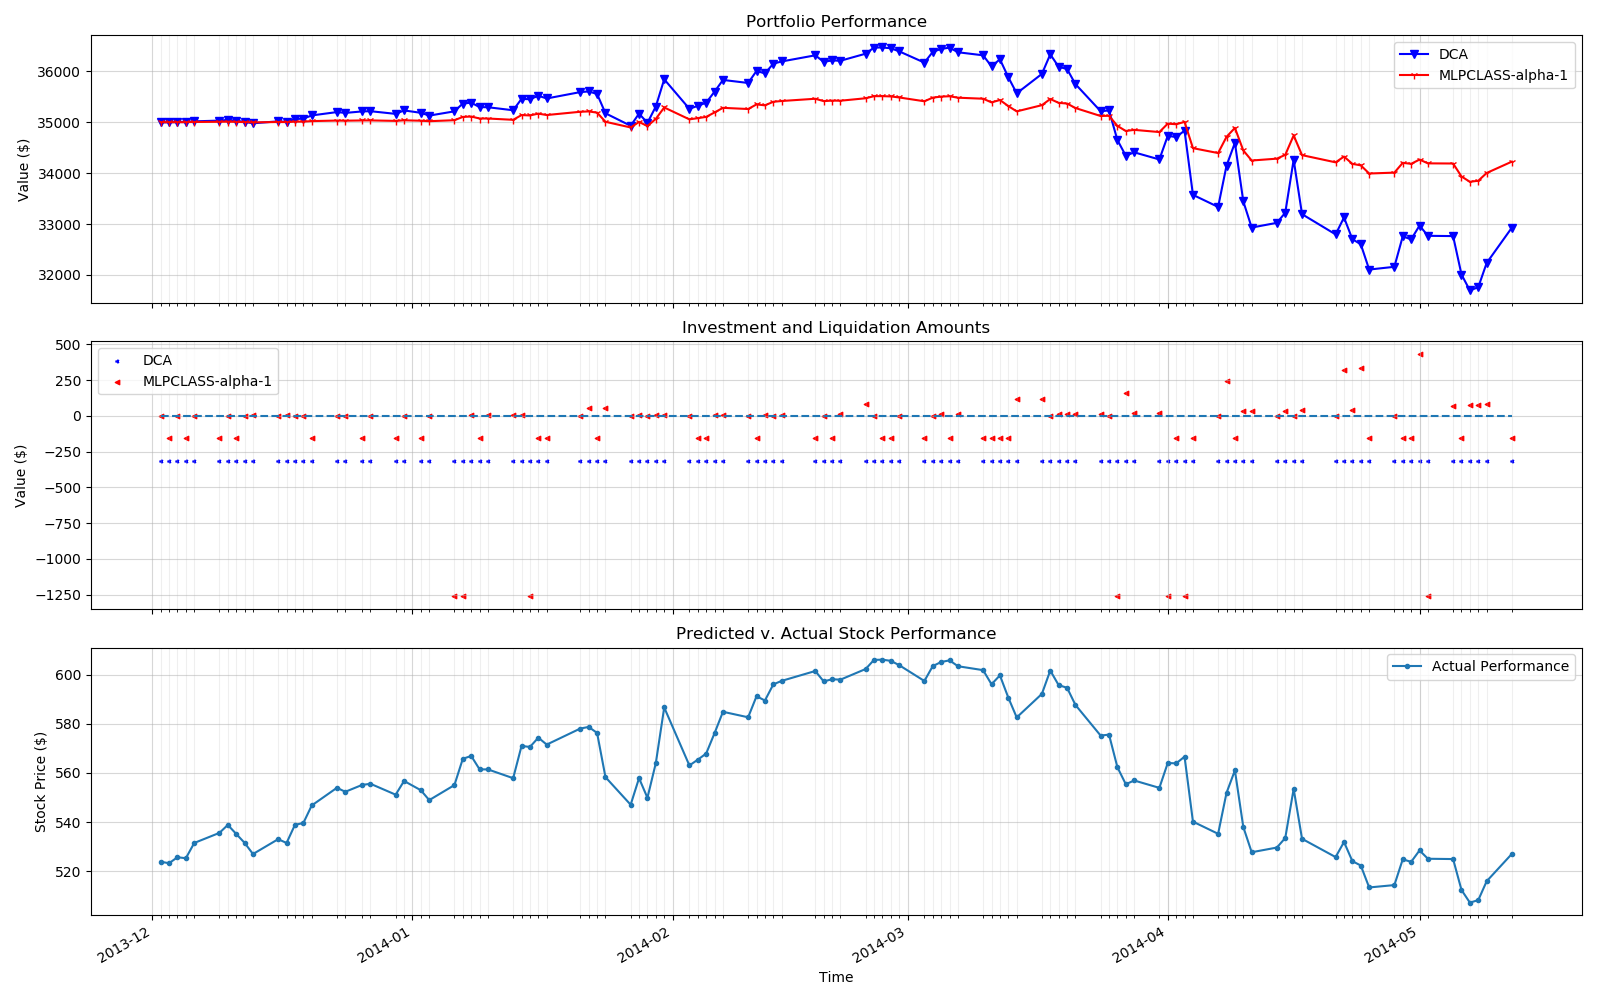
\includegraphics[width=\linewidth]{../Results/GOOG-DCA-MLPCLASS-2013-12-02--2014-05-12-alphas--[1]-train_length--1-performanceplot}
	\caption{This shows the multi layer perceptron classifier run on Google's stock over a time period in which the stock started and ended at the same point. Both investment strategies lost money, but the classifier-informed strategy outperformed DCA by \$10000 over the span of 5 months.}
	\label{class-steady}
\end{figure}


Ultimately, the performance of our strategy depended on certain hyper-parameters. The most important of these was the amount to invest. If the classifier predicted an increase or decrease, how much of the daily allotted amount should be spent. A more aggressive strategy was necessary to outperform dollar cost averaging in a bull market; however, this same aggressive strategy made our strategy perform worse than dollar cost averaging in a bearish market.

\section{Future Work}
TBD

\newpage
\appendix

\section{Pulling Data}
%\lstinputlisting[language=Python]{C:/Users/x92423/Documents/ThesisDataGrab/apiYahoo3.py}
%\lstinputlisting[language=Python]{C:/Users/x92423/Documents/ThesisDataGrab/dataMunch.py}
\begin{comment} 
\section{Pseudocode}
\begin{algorithmic}
	\ForAll{models}
		\ForAll{days}
			predictedYield $\gets predict(model, day)$
			principal += \Call{BuyOrSell}{predictedYield, dailyLimit, stockOwned}
		\EndFor 
	\EndFor 
	\Function{BuyOrSell}{predictedYield, dailyLimit, stockOwned}
		\If {$predictedYield > 0}
			x $\gets$ \Call{Buy}{predictedYield*dailyLimit}
		\EndIf
		\Else 
			x $\gets$ \Call{Sell}{predictedYield*stockOwned}
		\Return x
	\EndFunction 
\end{algorithmic}

\end{comment}
\begin{comment}

My results this semester are encouraging. We are able to outperform dollar cost averaging in a zero-gain market as well as a crashing market using the neural network model.

\subsection{Futility of Linear Models}
The linear models in general are insufficient in predicting stock performance. This was apparent when we found the model had a negative correlation. In other words, it would have been better for us to guess the stock would stay the same. Our model predicts very small increases and decreases with seemingly equal probability. The result of this is the simulation maintaining very small amounts of stock; almost all of the principal is not invested. The simulation invests a little, and then sells a little, which leads to a consistent return of 0\%. While this is better than losing money, this is an unsuccessful strategy and certainly worse than dollar cost averaging.

This can be seen in Figures \ref{crash}, \ref{increase}, and \ref{steady}. The portfolio value for the linear regression is flat over time, and you can see the buy/sell amounts randomly scattered about the zero line.

There are a few conclusions for why this may be the case:
\begin{itemize}
	\item Financial market data is too complicated to be encapsulated by such a vanilla model. Perhaps a linear model could be effective if we performed a significant amount of feature engineering. In other words, we would need to provide more than simply the time-lagged close price data for a linear model to have any chance of being successful.
	\item Prediction is difficult in this context. Perhaps it is a more auspicious pursuit to simply predict whether the stock will go up or down, rather than trying to pick exactly what the price will be. Reformulating the problem as a classification rather than a regression seemed like a good idea. We pursued this a little bit with similar results. This is a possibility for future exploration. 
\end{itemize}

\subsection{Difficulty Fitting Data with Neural Networks}
Specifically with the neural network, there were issues fitting the data. When attempting to find the weights through back propagation, the values did not converging. In order to get the values to converge, we had to seriously reduce the training set. This is bad when using neural networks, which are effective at using large datasets. Instead, because of time constraints and also the difficulty in creating a regression model given limited data, we choose a training data set of around 100. In the future, we need to rectify this issue to better take advantage of the full training set. This may require looking into sklearn's multi-layer perceptron regressor and the specific warning provided.

\subsection{Difficulties Comparing Results}
Dollar cost averaging is the baseline for the experiment. The goal is to beat dollar cost averaging with a strategy informed by machine learning. There are a few issues with the strategy that make the comparison difficult listed below:

\begin{itemize}
	\item Dollar cost averaging (DCA) does not factor in any sales. So, our investment strategy will be able to make gains when the stock ends at the same value it is purchased at as long as their is noise in between, whereas DCA will not make noticeable gains. Moreover, if the stock market decreases, our strategy has a chance to not invest or liquidate assets while DCA cannot. This makes it a somewhat unfair comparison for these two cases. 
	
	One might suggest comparing DCA and our strategy when the stock market increases, but this seems unfair to our strategy. It is a tough baseline to beat because DCA is at its best when you know the stock market is going to increase.
	
	\item The other issue with our strategy is when it comes to selling. We buy a proportion of our daily allotment $d$. However, we sell a proportion of our total purchased stock. If we currently have many shares of the stock, a confident projection that the market is going to decrease will lead to our strategy divesting a large proportion of its assets. It's kept from spending all of its money but not from selling all of its stocks.
	\item Finally, allocating a daily allotment $d$ might be hindering performance. The strategy is handicapped because it cannot get in early. For example, if the market is going to increase a lot, we will not be heavily invested at the beginning because we can only invest $d$ each day. As it is now, it would take a very confident prediction upwards for the strategy to invest the full $d$ dollars.  Meanwhile, DCA will blindly invest every period. Note: If our strategy were to confidently predict the stock to go up every day, it would be equivalent to using DCA to invest every day. One may counter that this isn't a disadvantage for our strategy because we can capitalize on local minimums/maximums in a way that DCA cannot, but the benefit of this is not obvious in practice.
\end{itemize}

\subsection{Summary of Results}
\textbf{Linear Models.} The linear models we tried did not fit the data in any meaningful way. We observed negative correlations for many fits suggesting a useless model. There is thought that a linear model could work but with more indicative features.

\textbf{Neural Network.} The neural network was our most effective model. It can outperform DCA when the stock decreases or stays the same, but loses big when the stock increases. The neural network predictor is poor as evidenced by the inability for weights to converge. This suggests the need for more predictive features. 

\textbf{ARIMA.} We attempted to use the conventional method for time series analysis, ARIMA. The issue with this was that a financial market expressed as a time series violates the stationarity requirements for ARIMA. This would not be an issue typically because you can decompose the model and transform it into one for which you could apply ARIMA. However, in testing many different datasets, it is not feasibly to transform each dataset so that it can work with ARIMA. However, this is something we can explore.

\section{Plan Moving Forward}
Moving forward, there are a number of things to address that can help improve our current prediction models. They are listed below in order of precedence.

\begin{enumerate}
	\item \textbf{Enforcing stationarity.} Stationarity is important. Reference Figure \ref{trend}. By training the model on one set of the data and applying it to another, later set, we assume that the model will be applicable. Consider training a model from Jan-49 to Jan-51. Now, apply the model from Jan-52 to Jan-54. We have trained the model on values between 2 and 2.2. Now, we are using the model to predict values between 2.2 to 2.4. We need to enforce stationarity on our financial data. The best way to do this is by time differencing. This will be the first focus of the rest of the project.
	
	\begin{figure}
		\centering
		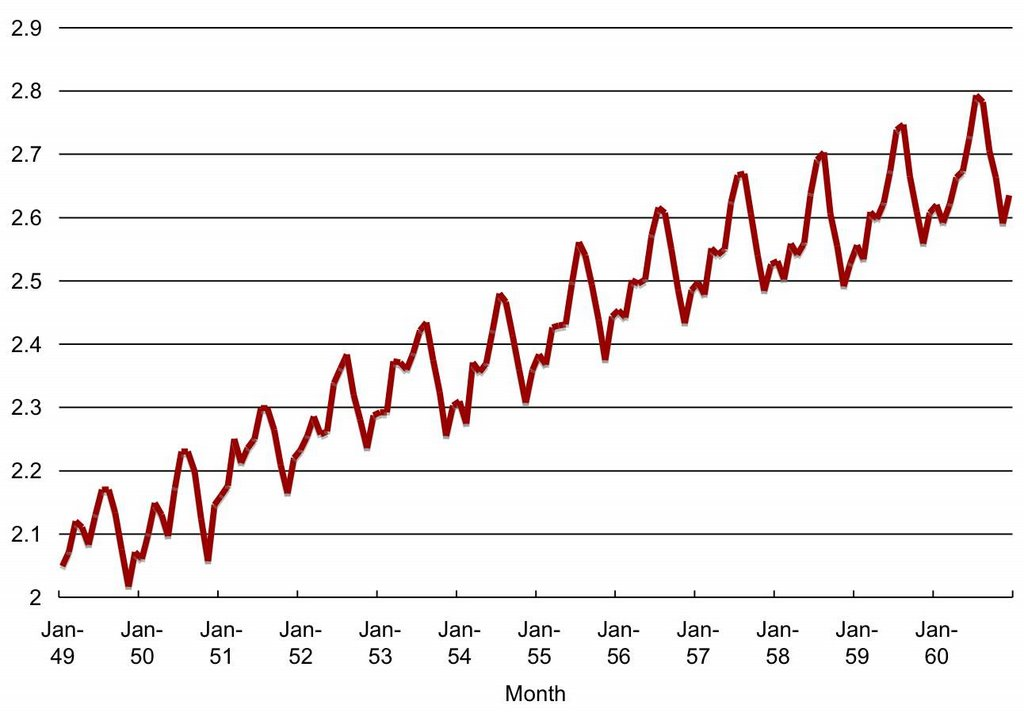
\includegraphics[width=.5\linewidth]{trend.jpg}
		\caption{This captures a time series with an upward trend. This is the problem with financial data. While the variation around the mean is often the same, there is a trend that confuses a model. Consider training a model from Jan-49 to Jan-51. Now, apply the model from Jan-52 to Jan-54. The model will be seeing values it has never seen before}
		\label{trend}
	\end{figure}

	\item \textbf{Fix the neural network.} We need to get the neural network working properly. In this case, there is a lot of available data and the neural network cannot take advantage of it. We think this problem is related to the non-stationary data, so hopefully once we address the first problem, the neural network will work better. We will also play with the learning rate of the neural network to force weight convergence.
	
	\item \textbf{Implement a recurrent neural network.} The plan is to try using a recurrent neural network (RNN) and see how that works. RNNs feed their output back through the input. The hope is that they can capture long term trends in addition to short term. This may increase our predicting accuracy.
	
	\item \textbf{Explore modifying strategy for classification and compare results to regression.} As previously mentioned, classification may be more auspicious than regression. We will need to modify the current investment strategy as well as reformulate the data as a classification problem. 
\end{enumerate}

\section{Conclusion}
Through a semester's work, we have taken major steps toward beating dollar cost averaging. We can pull historical stock data from the Internet, train a number of machine learning models to the data, and then run an investing simulation given a original investment strategy. The library of code can be found at this \href{https://github.com/jschless/thesis}{Git Repository}. 

While we have accomplished a lot, we have little to show for it as far as results. We will not be getting rich off of the model right now, but the hope is to refine and tune the model so we will be rich in the future. The shortcomings of the current system suggests a path ahead, which we will aggressively pursue in the following semester. It seems clear that this is an ambitious project, one tackled by hundreds of hedge-funds and quants with varying levels of success.

\clearpage 
\appendix

\section{Figures}
\begin{figure}[ht]
	\centering
	\makebox[\textwidth]{\includegraphics[width=1.2\linewidth]{../MidyearReport/crash.png}}
	\caption{This graph depicts the stock performance of Google over a market crash from November 2007 to November 2008. The bottom graph shows the actual stock performance in blue and the predicted performance by the ridge and multi-layer perceptron (MLP) models. Dollar cost averaging performs poorly (mirroring the market). Ridge stays stagnant as it does not maintain much stock at all. The MLP model owns stock but is able to divest later and therefore cuts its losses while DCA stays in for the long haul.}
	\label{crash}
\end{figure}

\begin{figure}[ht]
	\centering
	\makebox[\textwidth]{\includegraphics[width=1.2\linewidth]{../MidyearReport/steady.png}}
	
	\caption{This graph depicts the stock performance of Google over a market that changes around but ultimately ends where it started. The time period is from December 2013 to May 2014. The bottom graph shows the actual stock performance in blue and the predicted performance by the ridge and multi-layer perception (MLP) models. Dollar cost averaging barely makes any money (mirroring the market). Although it appears to go down, it only looses \$400. Ridge stays stagnant as it does not maintain much stock at all. The MLP model breaks even earning \$200 over the course of the six months.}
	\label{steady}
\end{figure}

\begin{figure}[ht]
	\centering
	\makebox[\textwidth]{\includegraphics[width=1.2\linewidth]{../MidyearReport/increase.png}}	
	\caption{This graph depicts the stock performance of Google over a booming market from November 2014 to November 2015. The bottom graph shows the actual stock performance in blue and the predicted performance by the ridge and multi-layer perceptron (MLP) models. Dollar cost averaging performs well and increases significantly with the market. Ridge stays stagnant again. The MLP model goes positive earning approximately \$500, but cannot compete with DCA which earns \$2000 over the year.}
	\label{increase}
\end{figure}

\end{comment}

\clearpage 
\bibliographystyle{alpha}
\bibliography{litreview}
\end{document}
